\input{kapittel}

\kapittel{4}{Vektorer}
\label{ch:vektorer}

Nå har vi funnet ut nøyaktig hvordan vi kan løse et hvilket som helst
lineært likningssystem.  Så på sett og vis kunne vi sagt oss ferdige
med lineære likningssystemer nå.  Det skal vi ikke gjøre.

Det er selvfølgelig veldig flott at vi har en løsningsmetode som
alltid fungerer.  Men det finnes mange mye mer spennende ting vi kan
få ut av å holde på med lineære likningssystemer enn det å finne
løsningene -- vi må bare betrakte dem på den rette måten.

Fra dette kapitlet av skal vi begynne å innføre konsepter og notasjon
som gjør oss i stand til å se på et likningssystem ikke bare som en
drøss forskjellige likninger, men som én enkelt likning.  Denne
endringen av perspektiv gjør at vi får et helt annet bilde av hva et
lineært likningssystem er for noe, og vi får muligheten til å stille
helt nye spørsmål -- og besvare dem.


\section*{To visualiseringer av et likningssystem}

Hvis vi har et lineært likningssystem med to likninger og to ukjente,
så kan vi tegne grafene til likningene (det blir to rette linjer) og
finne punktet der de krysser hverandre (det er løsningen av systemet).
For eksempel vil systemet
\[
\systeme{
5x + 2y = 11,
3x + 4y = 8
}
\]
gi opphav til denne tegningen:
\begin{center}
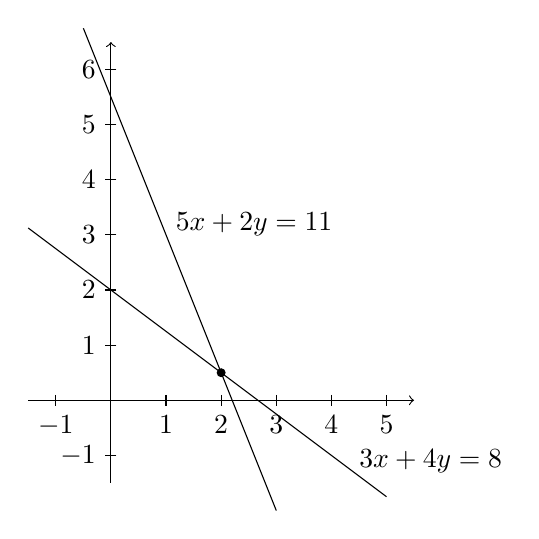
\begin{tikzpicture}[scale=.7]
\draw[->] (-1.5,0) -- (5.5,0);
\draw[->] (0,-1.5) -- (0,6.5);
\foreach \x in {-1,1,2,...,5}
\draw (\x,.1) -- (\x,-.1) node[anchor=north] {$\x$};
\foreach \y in {-1,1,2,...,6}
\draw (.1,\y) -- (-.1,\y) node[anchor=east] {$\y$};
\draw (-.5,6.75) -- (3,-2); % y = 11/2 - (5/2)x
\node[anchor=west] at (1,3.2) {$5x + 2y = 11$};
\draw (-1.5,3.125) -- (5,-1.75); % y = 2 - (3/4)x
\node at (5.8,-1.1) {$3x + 4y = 8$};
\filldraw (2,.5) circle [radius=2pt];
\end{tikzpicture}
\end{center}
Men det går også an å visualisere det samme likningssystemet på en
helt annen måte.  Vi kan si at vi gikk \emph{radvis} gjennom systemet
for å lage tegningen over: Vi så på én og én «rad» (likning) i
systemet, og tegnet grafen dens.  Men vi kan også gå gjennom systemet
\emph{kolonnevis}.
\[
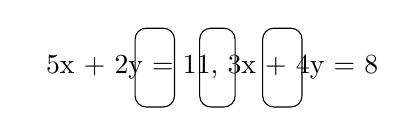
\begin{tikzpicture}
\node at (0,0) {\systeme{
5x + 2y = 11,
3x + 4y = 8
}};
\draw[rounded corners] (-.92,-.5) -- (-.92,.5) -- (-.42,.5) -- (-.42,-.5) -- cycle;
\draw[rounded corners] (-.1,-.5) -- (-.1,.5) -- (.35,.5) -- (.35,-.5) -- cycle;
\draw[rounded corners] (.7,-.5) -- (.7,.5) -- (1.2,.5) -- (1.2,-.5) -- cycle;
\end{tikzpicture}
\]
Første kolonne består av de to $x$-leddene:
\[
\vv{5x}{3x}
\]
Hvis vi setter inn en verdi for~$x$, så får vi to konkrete tall i
kolonnen.  Hvis vi for eksempel setter inn $x=2$, så får vi:
\[
\vv{10}{6}
\]
Denne tingen som består av to tall kaller vi en \emph{vektor} (eller
vi kan si \emph{kolonnevektor} for å fremheve det at vi skriver
tallene nedover i en kolonne).  Siden den består av to tall, er det en
åpenbar måte å tegne den på: som et punkt i planet.  Det første tallet
er~$10$ og det andre er~$6$ -- dermed går vi til punktet som er $10$
enheter bortover på førsteaksen og $6$ enheter oppover på andreaksen:
\begin{center}
\begin{tikzpicture}[scale=.55]
\draw[->] (-1.5,0) -- (11.5,0);
\draw[->] (0,-1.5) -- (0,6.5);
\foreach \x in {-1,...,11}
\draw (\x,.1) -- (\x,-.1);
\foreach \x in {-1,1,2,...,11}
\node[anchor=north] at (\x,-.1) {$\x$};
\foreach \y in {-1,...,6}
\draw (.1,\y) -- (-.1,\y);
\foreach \y in {-1,1,2,...,6}
\node[anchor=east] at (-.1,\y) {$\y$};
%%%%
\filldraw (10,6) circle [radius=2pt];
\draw[dashed,gray] (10,0) -- (10,6) -- (0,6);
\end{tikzpicture}
\end{center}
Denne vektoren representerer én mulighet for verdiene av $x$-leddene i
de to likningene.  Ved å sette inn andre verdier for~$x$, kan vi finne
andre muligheter.  Om vi setter inn $x=-1$, eller $x=\frac{1}{5}$,
eller $x=3$, får vi
\[
\vv{-5}{-3},\quad\text{eller}\quad
\vv{1}{3/5},\quad\text{eller}\quad
\vv{15}{9}.
\]
La oss tegne disse vektorene også som punkter:
\begin{center}
\begin{tikzpicture}[scale=.38]
\draw[->] (-5.5,0) -- (15.5,0);
\draw[->] (0,-3.5) -- (0,9.5);
\foreach \x in {-5,...,15}
\draw (\x,.1) -- (\x,-.1);
\foreach \x in {-5,5,10,15}
\node[anchor=north] at (\x,-.1) {$\x$};
\foreach \y in {-3,...,9}
\draw (.1,\y) -- (-.1,\y);
\foreach \y in {5}
\node[anchor=east] at (-.1,\y) {$\y$};
%%%%
\filldraw (10,6) circle [radius=2pt];
\filldraw (-5,-3) circle [radius=2pt];
\filldraw (1,.6) circle [radius=2pt];
\filldraw (15,9) circle [radius=2pt];
\end{tikzpicture}
\end{center}
Nå legger du muligens merke til at alle punktene våre ligger på en
rett linje, og det er ikke så rart.  Vi kan tenke på alle disse
vektorene som \emph{skaleringer} av denne vektoren:
\[
\vv{5}{3}
\]
For å se hva det vil si å skalere en vektor, kan det være praktisk å
tegne vektorene på en litt annen måte, nemlig som piler.  Istedenfor å
tegne vektoren~$\vvS{5}{3}$ som en prikk plassert i koordinatene
$(5,3)$, kan vi tegne den som en pil fra origo til dette punktet:
\begin{center}
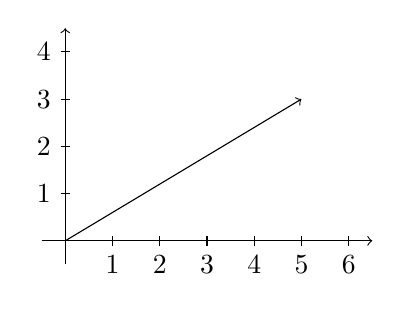
\begin{tikzpicture}[scale=.6]
\draw[->] (-.5,0) -- (6.5,0);
\draw[->] (0,-.5) -- (0,4.5);
\foreach \x in {1,...,6}
\draw (\x,.1) -- (\x,-.1) node[anchor=north] {$\x$};
\foreach \y in {1,...,4}
\draw (.1,\y) -- (-.1,\y) node[anchor=east] {$\y$};
%%%%
\draw[->] (0,0) -- (5,3);
\end{tikzpicture}
\end{center}
Å skalere vektoren blir det samme som å strekke ut pilen slik at den
får en annen lengde, men fremdeles peker i samme retning.  Hvis vi
skalerer den med~$3$, blir den tre ganger så lang.  Hvis vi skalerer
den med~$1/2$, blir den halvparten så lang.

Vi skriver
\[
\vv{5}{3} \cdot x
\]
for «vektoren~$\vvS{5}{3}$ skalert med tallet~$x$», og da har vi:
\[
\vv{5}{3} \cdot x = \vv{5x}{3x}
\]
Vi bruker altså et gangetegn for å symbolisere skalering av en vektor,
og vi kan også velge å si at vi \emph{ganger} vektoren med~$x$,
istedenfor å si at vi skalerer den.  Akkurat som med vanlig ganging
kan vi dessuten velge å utelate gangetegnet:
\[
\vv{5}{3} x
\]

Her er noen skaleringer av vektoren~$\vvS{5}{3}$, tegnet som piler:
\begin{center}
\begin{tikzpicture}[scale=.6]
\draw[->] (-.5,0) -- (11.5,0);
\draw[->] (0,-.5) -- (0,7.5);
\foreach \x in {1,...,11}
\draw (\x,.1) -- (\x,-.1) node[anchor=north] {$\x$};
\foreach \y in {1,...,7}
\draw (.1,\y) -- (-.1,\y) node[anchor=east] {$\y$};
%%%%
\draw[->] (0,0) -- (5,3) node[anchor=south east] {$\vv{5}{3}$};
\draw[->] (0,0) -- (10,6) node[anchor=north west] {$\vv{5}{3} \cdot 2$};
\draw[->] (0,0) -- (2.5,1.5) node[anchor=south east] {$\vv{5}{3} \cdot \frac{1}{2}$};
\end{tikzpicture}
\end{center}

Hva om vi skalerer vektoren med et negativt tall?  Om vi for eksempel
ganger med~$-1$, så får vi:
\[
\vv{5}{3} \cdot (-1) = \vv{5 \cdot (-1)}{3 \cdot (-1)} = \vv{-5}{-3}
\]
Vi kan tegne opp dette også:
\begin{center}
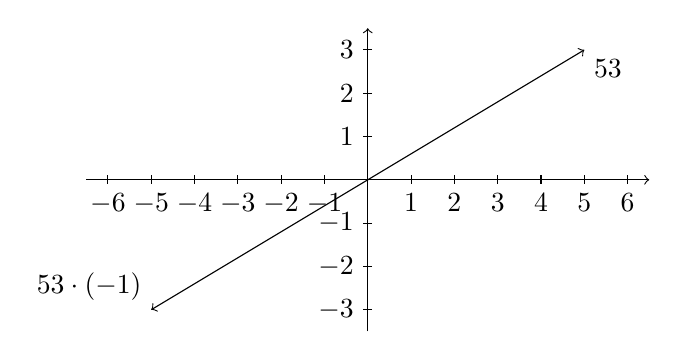
\begin{tikzpicture}[scale=.55]
\draw[->] (-6.5,0) -- (6.5,0);
\draw[->] (0,-3.5) -- (0,3.5);
\foreach \x in {-6,...,-1,1,2,...,6}
\draw (\x,.1) -- (\x,-.1) node[anchor=north] {$\x$};
\foreach \y in {-3,...,-1,1,2,3}
\draw (.1,\y) -- (-.1,\y) node[anchor=east] {$\y$};
%%%%
\draw[->] (0,0) -- (5,3) node[anchor=north west] {$\vv{5}{3}$};
\draw[->] (0,0) -- (-5,-3) node[anchor=south east] {$\vv{5}{3} \cdot (-1)$};
\end{tikzpicture}
\end{center}
Det er altså ikke helt sant som vi sa tidligere at en skalert vektor
peker i samme retning som den opprinnelige vektoren.  Eller kanskje vi
kan si at det kommer litt an på nøyaktig hva man mener med «samme
retning».  Når vi ganger en vektor med et negativt tall, så får vi en
ny vektor som peker i \emph{stikk motsatt retning} -- og hvis vi vil,
så kan vi velge å tenke på det som «samme retning, men med motsatt
fortegn».

Hvis vi nå vil se på alle mulige skaleringer av vektoren~$\vvS{5}{3}$,
så får vi alle punktene på denne rette linjen:
\begin{center}
\begin{tikzpicture}[scale=.6]
\draw[->] (-6.5,0) -- (6.5,0);
\draw[->] (0,-3.5) -- (0,3.5);
\foreach \x in {-6,...,-1,1,2,...,6}
\draw (\x,.1) -- (\x,-.1) node[anchor=north] {$\x$};
\foreach \y in {-3,...,-1,1,2,3}
\draw (.1,\y) -- (-.1,\y) node[anchor=east] {$\y$};
%%%%
\draw (-5,-3) -- (5,3);
\end{tikzpicture}
\end{center}
Her har vi gått over til å tegne hver vektor som et punkt igjen,
istedenfor å tegne piler.  Her snakker vi jo om uendelig mange
vektorer, og det ville bare blitt rot om vi skulle prøve å tegne
uendelig mange piler.  Men uendelig mange punkter går helt fint å
tegne -- det blir ganske enkelt en linje.

Generelt vil vi gi oss selv fullstendig frihet til å tegne vektorer
som enten punkter eller piler, alt etter hva som passer best i den
aktuelle sammenhengen.

Men la oss nå gå tilbake til det vi startet hele denne diskusjonen
med, nemlig dette likningssystemet:
\[
\systeme{
5x + 2y = 11,
3x + 4y = 8
}
\]
Nå har vi tegnet opp en linje som representerer alle muligheter for
verdiene i den første kolonnen av systemet ($x$-leddene).  Hvis vi
gjør det samme med den andre kolonnen også, så har vi disse to
linjene:
\begin{center}
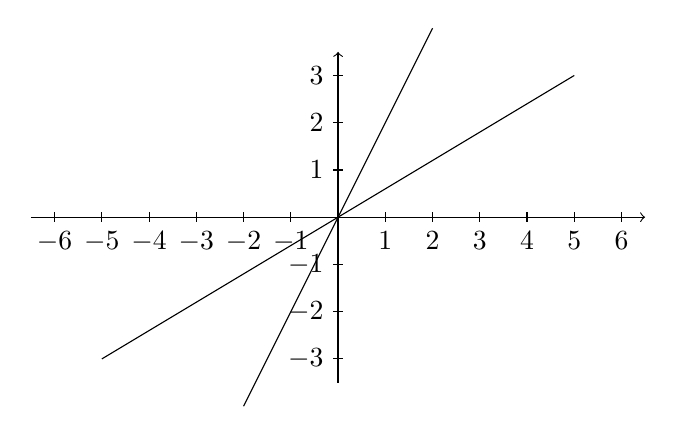
\begin{tikzpicture}[scale=.6]
\draw[->] (-6.5,0) -- (6.5,0);
\draw[->] (0,-3.5) -- (0,3.5);
\foreach \x in {-6,...,-1,1,2,...,6}
\draw (\x,.1) -- (\x,-.1) node[anchor=north] {$\x$};
\foreach \y in {-3,...,-1,1,2,3}
\draw (.1,\y) -- (-.1,\y) node[anchor=east] {$\y$};
%%%%
\draw (-5,-3) -- (5,3);
\draw (-2,-4) -- (2,4);
\end{tikzpicture}
\end{center}
Vi må passe på litt så vi ikke forvirrer oss selv når vi prøver å
forstå hva vi ser på denne tegningen.  Vi er vant til å tenke på den
horisontale aksen som «$x$-aksen» og den vertikale som «$y$-aksen»,
men det kan vi ikke gjøre nå.  Nå er det sånn at hvor langt vi går
bortover langs førsteaksen handler om hvilket tall vi har i den første
likningen, og hvor høyt vi går oppover på andreaksen handler om
hvilket tall vi har i den andre likningen.
Vi kan kalle de to likningene våre for likning~\En{} og likning~\To:
\[
\systeme{
\makebox[0pt][l]{\hspace{-2em}\En} 5x + 2y = 11,
\makebox[0pt][l]{\hspace{-2em}\To} 3x + 4y = 8
}
\]
Da kan vi markere aksene slik som dette (dersom vi vil markere dem med
noe i det hele tatt -- vanligvis lar vi det bare være underforstått
hva aksene står for):
\begin{center}
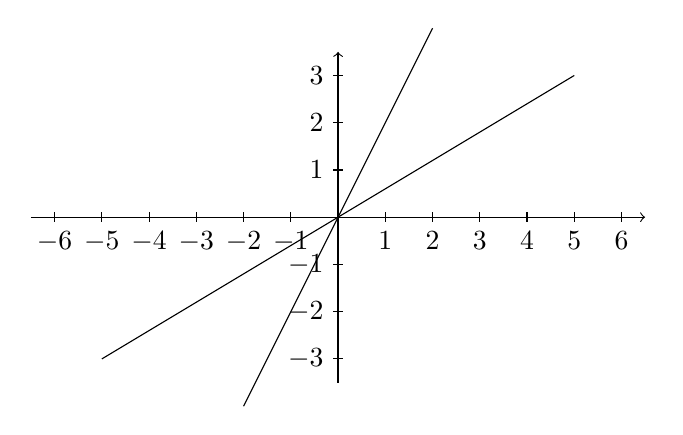
\begin{tikzpicture}[scale=.6]
\draw[->] (-6.5,0) -- (6.5,0) node[anchor=south] {\En};
\draw[->] (0,-3.5) -- (0,3.5) node[anchor=west] {\To};
\foreach \x in {-6,...,-1,1,2,...,6}
\draw (\x,.1) -- (\x,-.1) node[anchor=north] {$\x$};
\foreach \y in {-3,...,-1,1,2,3}
\draw (.1,\y) -- (-.1,\y) node[anchor=east] {$\y$};
%%%%
\draw (-5,-3) -- (5,3);
\draw (-2,-4) -- (2,4);
\end{tikzpicture}
\end{center}
Men hvor på denne tegningen kan vi finne løsningen av
likningssystemet?  Det er det ikke så lett å få øye på.

Det blir litt tydeligere hvis vi tegner opp de to koeffisientvektorene
som piler, og «målet» -- altså høyresiden av likningene -- som et punkt:
\begin{center}
\begin{tikzpicture}[scale=.6]
\draw[->] (-.5,0) -- (11.5,0);
\draw[->] (0,-.5) -- (0,8.5);
\foreach \x in {1,2,...,11}
\draw (\x,.1) -- (\x,-.1) node[anchor=north] {$\x$};
\foreach \y in {1,2,...,8}
\draw (.1,\y) -- (-.1,\y) node[anchor=east] {$\y$};
%%%%
\draw[->] (0,0) -- (5,3) node[anchor=north west] {$\vv{5}{3}$};
\draw[->] (0,0) -- (2,4) node[anchor=south east] {$\vv{2}{4}$};
\filldraw (11,8) circle [radius=2pt] node[anchor=north east] {$\vv{11}{8}$};
\end{tikzpicture}
\end{center}
Det å finne en løsning av systemet er det samme som å svare på dette
spørsmålet: Kan vi skalere de to koeffisientvektorene med hvert sitt
tall ($x$ og~$y$), og deretter legge dem sammen, slik at resultatet
blir høyresidevektoren?

Før vi kan svare på det spørsmålet, må vi bestemme oss for hva vi
mener med å \emph{legge sammen} to vektorer.  Vi vil at dette skal
stemme overens med det som skjer i likningssystemet vårt, så vi vil at
\[
\vv{5}{3} x + \vv{2}{4} y
\qquad\text{skal være lik}\qquad
\vv{5x + 2y}{3x + 4y}
\]
Derfor bestemmer vi at når vi skal legge sammen to vektorer, så legger
vi de øverste tallene i hver vektor sammen med hverandre, og så legger
vi de nederste tallene i hver vektor sammen med hverandre:
\[
\vv{a}{b} + \vv{c}{d} = \vv{a+c}{b+d}
\]

Akkurat som med skalering, kan også addisjon av vektorer gjøres på en
fin geometrisk måte med piler.  Vi kan tenke at vi først følger den
ene pilen og så den andre -- da må vi bare først ha flyttet den andre
pilen slik at den starter der hvor den første slutter.  Stedet vi
ender opp er summen av vektorene.  Hvis vi vil legge sammen
vektorene~$\vvS{5}{3}$ og~$\vvS{2}{4}$, så ser det slik ut:
\begin{center}
\begin{tikzpicture}[scale=.6]
\draw[->] (-.5,0) -- (11.5,0);
\draw[->] (0,-.5) -- (0,8.5);
\foreach \x in {1,2,...,11}
\draw (\x,.1) -- (\x,-.1) node[anchor=north] {$\x$};
\foreach \y in {1,2,...,8}
\draw (.1,\y) -- (-.1,\y) node[anchor=east] {$\y$};
%%%%
\draw[->] (0,0) -- (5,3) node[anchor=north west] {$\vv{5}{3}$};
\draw[->] (0,0) -- (2,4) node[anchor=south east] {$\vv{2}{4}$};
\draw[->,dashed] (5,3) -- (7,7) node[anchor=west] {$\vv{5}{3} + \vv{2}{4} = \vv{7}{7}$};
\end{tikzpicture}
\end{center}
Vi får selvfølgelig samme resultat uansett hvilken av de to vektorene
vi følger først, og hvilken vi flytter slik at den kommer etterpå.  En
annen måte å tegne det samme på, uten å måtte si at én vektor kommer
først og den andre sist, er å tegne et parallellogram der de to
vektorene som skal legges sammen utgjør to av sidene:
\begin{center}
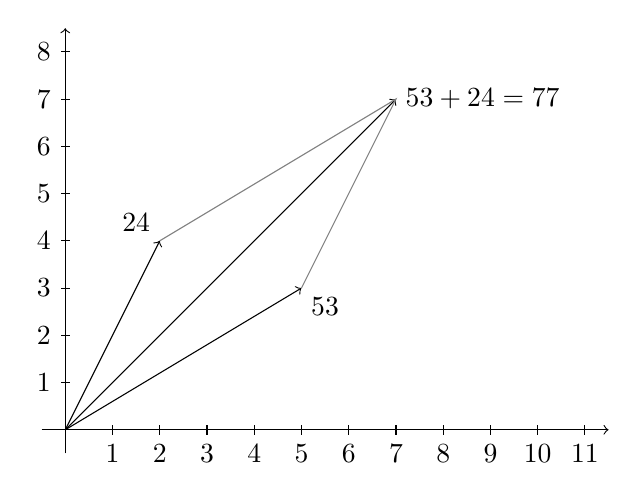
\begin{tikzpicture}[scale=.6]
\draw[->] (-.5,0) -- (11.5,0);
\draw[->] (0,-.5) -- (0,8.5);
\foreach \x in {1,2,...,11}
\draw (\x,.1) -- (\x,-.1) node[anchor=north] {$\x$};
\foreach \y in {1,2,...,8}
\draw (.1,\y) -- (-.1,\y) node[anchor=east] {$\y$};
%%%%
\draw[->] (0,0) -- (5,3) node[anchor=north west] {$\vv{5}{3}$};
\draw[->] (0,0) -- (2,4) node[anchor=south east] {$\vv{2}{4}$};
\draw[->] (0,0) -- (7,7) node[anchor=west] {$\vv{5}{3} + \vv{2}{4} = \vv{7}{7}$};
\draw[gray] (5,3) -- (7,7) -- (2,4);
\end{tikzpicture}
\end{center}

Nå som vi har klart for oss hva det vil si å legge sammen vektorer,
kan vi vende tilbake til å se etter løsningen på likningssystemet.
Når vi bare la sammen de to vektorene våre, så havnet vi altså i
punktet~$(7,7)$.  For å løse systemet, må vi skalere opp de to
vektorene med hvert sitt tall $x$ og~$y$ slik at vi isteden ender opp
i punktet~$(11,8)$.

Vi kan prøve oss frem med noen ulike verdier for $x$ og~$y$.  Hvis vi
setter inn $0$, $1$ eller~$2$ for $x$ og for~$y$, så kommer vi til de
forskjellige hjørnene i dette rutenettet:
% {\small
% \begin{align*}
% \vv{5}{3} \cdot 0 + \vv{2}{4} \cdot 0 &= \vv{0}{0}
% &\qquad
% \vv{5}{3} \cdot 0 + \vv{2}{4} \cdot 0 &= \vv{0}{0}
% \end{align*}
% }
\begin{center}
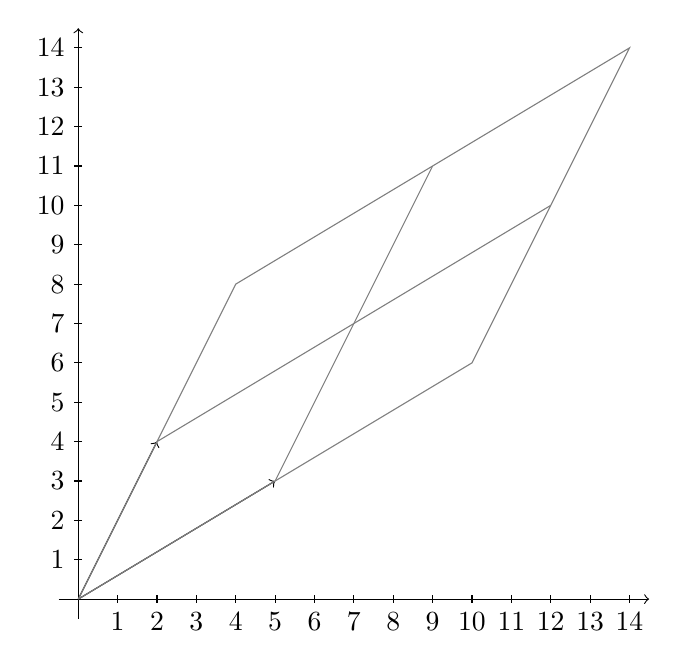
\begin{tikzpicture}[scale=.5]
\draw[->] (-.5,0) -- (14.5,0);
\draw[->] (0,-.5) -- (0,14.5);
\foreach \x in {1,2,...,14}
\draw (\x,.1) -- (\x,-.1) node[anchor=north] {$\x$};
\foreach \y in {1,2,...,14}
\draw (.1,\y) -- (-.1,\y) node[anchor=east] {$\y$};
%%%%
\draw[->] (0,0) -- (5,3);
\draw[->] (0,0) -- (2,4);
\draw[gray] (0,0) -- (10,6) -- (14,14) -- (4,8) -- (0,0);
\draw[gray] (5,3) -- (9,11);
\draw[gray] (2,4) -- (12,10);
%\filldraw (11,8) circle [radius=2pt] node[anchor=north east] {$\vv{11}{8}$};
\end{tikzpicture}
\end{center}
Hvis du finner frem til punktet $(11,8)$ på denne tegningen, så ser du
at det ligger midt mellom
\[
\vv{5}{3} \cdot 2 + \vv{2}{4} \cdot 0
\qquad\text{og}\qquad
\vv{5}{3} \cdot 2 + \vv{2}{4} \cdot 1.
\]
Da kan vi gjette at $x=2$ og $y=1/2$ er løsningen av likningen -- og
ganske riktig:
\[
\vv{5}{3} \cdot 2 + \vv{2}{4} \cdot \frac{1}{2}
= \vv{10}{6} + \vv{1}{2}
= \vv{11}{8}
\]
Vi fant altså løsningen.  Men det var ikke egentlig hovedpoenget her
-- poenget var å se at vi kan lage to radikalt forskjellige visuelle
fremstillinger av det samme likningssystemet:
\begin{center}
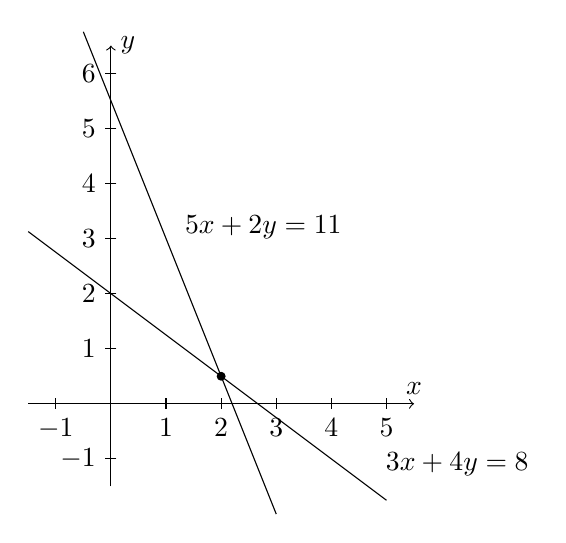
\begin{tikzpicture}[scale=.7]
\draw[->] (-1.5,0) -- (5.5,0) node[anchor=south] {$x$};
\draw[->] (0,-1.5) -- (0,6.5) node[anchor=west] {$y$};
\foreach \x in {-1,1,2,...,5}
\draw (\x,.1) -- (\x,-.1) node[anchor=north] {$\x$};
\foreach \y in {-1,1,2,...,6}
\draw (.1,\y) -- (-.1,\y) node[anchor=east] {$\y$};
\draw (-.5,6.75) -- (3,-2); % y = 11/2 - (5/2)x
\node[anchor=west] at (1,3.2) {\En{} $5x + 2y = 11$};
\draw (-1.5,3.125) -- (5,-1.75); % y = 2 - (3/4)x
\node at (6.2,-1.1) {\To{} $3x + 4y = 8$};
\filldraw (2,.5) circle [radius=2pt];
\end{tikzpicture}
\end{center}
\begin{center}
\begin{tikzpicture}[scale=.6]
\draw[->] (-.5,0) -- (11.5,0) node[anchor=south] {\En};
\draw[->] (0,-.5) -- (0,8.5) node[anchor=west] {\To};
\foreach \x in {1,2,...,11}
\draw (\x,.1) -- (\x,-.1) node[anchor=north] {$\x$};
\foreach \y in {1,2,...,8}
\draw (.1,\y) -- (-.1,\y) node[anchor=east] {$\y$};
%%%%
\draw[->] (0,0) -- (5,3) node[anchor=north west] {$\vv{5}{3}$};
\draw[->] (0,0) -- (2,4) node[anchor=south east] {$\vv{2}{4}$};
\filldraw (11,8) circle [radius=2pt] node[anchor=north east] {$\vv{11}{8}$};
\end{tikzpicture}
\end{center}

Disse to tegningene er tett knyttet sammen siden begge illustrerer det
samme likningssystemet.  Men det er likevel ikke så lett å se på
tegningene at de har noe med hverandre å gjøre.  Det er fordi
tegningene på sett og vis tilsvarer det å betrakte likningssystemet
fra to forskjellige synspunkter som står vinkelrett på hverandre.

Når du nå ser begge tegningene, så blir det kanskje klart hva vi mente
i begynnelsen av kapitlet med at vi lager den ene tegningen ved å gå
radvis gjennom likningssystemet, og den andre ved å gå kolonnevis.  I
den første tegningen ser vi hver rad -- altså hver likning -- som en
separat komponent; i den andre ser vi hver kolonne som en separat
komponent.

Hvilken av måtene vi visualiserer systemet på har konsekvenser for hva
slags spørsmål det blir naturlig å stille.  Tenk for eksempel på et
spørsmål som dette:
\begin{quote}
Hva skjer hvis vi bytter ut likning~\To{} med en annen likning?
\end{quote}
Om vi ser på den første tegningen, så er det veldig greit å tenke på
dette spørsmålet: Vi beholder grafen for likning~\En{} akkurat som den
er, og tegner en ny graf for likning~\To.  Men om vi ser på den andre
tegningen, så vil det å bytte ut likning~\To{} påvirke alle deler av
tegningen, så alt må tegnes på nytt.

Men så kan vi tenke på et annet spørsmål:
\begin{quote}
Hva skjer hvis vi bytter ut tallene på høyresiden av likningssystemet?
\end{quote}
Nå blir det helt omvendt.  Den første tegningen må tegnes helt på
nytt, siden tallene på høyresiden påvirker begge grafene.  Den andre
tegningen, derimot, kan enkelt modifiseres.  Begge de to pilene blir
værende akkurat som de er; vi bare flytter på målpunktet.

% Vi kan forfølge tanken fra dette siste spørsmålet litt videre: Kan det
% tenkes at det er noen muligheter for høyresiden som ville gjort at
% systemet ikke blir løsbart?  Hvis vi ser på den andre tegningen vår,
% så kan vi ganske raskt overbevise oss selv om at vi kan komme til et
% hvilket som helst punkt ved å kombinere de to vektorene $\vvS{5}{3}$
% og~$\vvS{2}{4}$ (husk at vi kan bruke både positive og negative tall
% til å skalere vektorene med).  Det betyr at uansett hvilke tall vi
% måtte putte på høyresiden, så blir systemet løsbart.  Denne (riktignok
% ikke veldig dype) innsikten kommer naturlig ved å se på det andre
% tegningen, men er overhodet ikke mulig å få øye på i den første.
%%%%%% TODO fiks ^ (eller bare ikke ta det med)

\section*{Vektorer i planet, rommet og videre}

La oss fortsette enda litt til med det samme likningssystemet vi har
sett på hittil i kapitlet:
\[
\systeme{
\makebox[0pt][l]{\hspace{-2em}\En} 5x + 2y = 11,
\makebox[0pt][l]{\hspace{-2em}\To} 3x + 4y = 8
}
\]
Vi skal prøve å endre systemet, og se hva slags konsekvenser
endringene får for de to måtene å tegne det på.

Først kan vi se hva som skjer hvis vi legger til en ukjent til, for
eksempel slik som dette:
\[
\systeme{
\makebox[0pt][l]{\hspace{-2em}\En} 5x + 2y -  z = 11,
\makebox[0pt][l]{\hspace{-2em}\To} 3x + 4y + 2z = 8
}
\]
Tegningen med vektorer kan enkelt og greit modifiseres tilsvarende --
det er bare å legge til en vektor til:
\begin{center}
\begin{tikzpicture}[scale=.55]
\draw[->] (-1.5,0) -- (11.5,0) node[anchor=south] {\En};
\draw[->] (0,-.5) -- (0,8.5) node[anchor=west] {\To};
\foreach \x in {-1,1,2,...,11}
\draw (\x,.1) -- (\x,-.1) node[anchor=north] {$\x$};
\foreach \y in {1,2,...,8}
\draw (.1,\y) -- (-.1,\y) node[anchor=east] {$\y$};
%%%%
\draw[->] (0,0) -- (5,3) node[anchor=north west] {$\vv{5}{3}$};
\draw[->] (0,0) -- (2,4) node[anchor=south east] {$\vv{2}{4}$};
\draw[->] (0,0) -- (-1,2) node[anchor=south east] {$\vv{-1}{2}$};
\filldraw (11,8) circle [radius=2pt] node[anchor=north east] {$\vv{11}{8}$};
\end{tikzpicture}
\end{center}
Tegningen med grafer, derimot, blir mer komplisert.  Nå kan vi ikke
lenger se på bare et todimensjonalt plan med en $x$- og en $y$-akse;
vi må ha et tredimensjonalt rom med $x$-, $y$- og $z$-akser.  Hver
likning beskriver ikke lenger en linje, men et plan.  Det blir ikke så
lett å tegne, men du kan (med litt innsats) lage en tredimensjonal
modell som viser planet som er beskrevet av likning~\En{} og det som
er beskrevet av likning~\To.  Du kan også lage en perspektivtegning
med tre akser, finne ut hvor hvert plan skjærer hver av aksene, og
bruke det til å se for deg omtrent hvordan de to planene ser ut.

Hva om vi isteden modifiserer systemet ved å legge til en ny likning?
For eksempel slik som dette:
\[
\systeme{
\makebox[0pt][l]{\hspace{-2em}\En}  5x + 2y = 11,
\makebox[0pt][l]{\hspace{-2em}\To}  3x + 4y = 8,
\makebox[0pt][l]{\hspace{-2em}\Tre} \phantom{3}x - 2y = 1
}
\]
Da blir situasjonen omvendt.  Tegningen med grafer blir latterlig
enkel å tilpasse -- vi tegner bare inn en ny graf:
\begin{center}
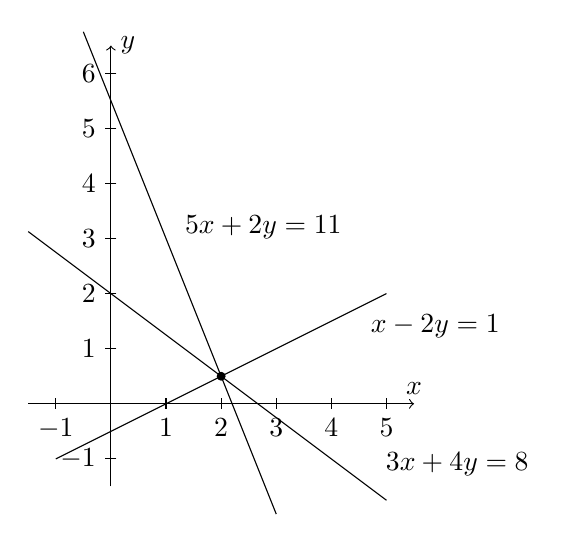
\begin{tikzpicture}[scale=.7]
\draw[->] (-1.5,0) -- (5.5,0) node[anchor=south] {$x$};
\draw[->] (0,-1.5) -- (0,6.5) node[anchor=west] {$y$};
\foreach \x in {-1,1,2,...,5}
\draw (\x,.1) -- (\x,-.1) node[anchor=north] {$\x$};
\foreach \y in {-1,1,2,...,6}
\draw (.1,\y) -- (-.1,\y) node[anchor=east] {$\y$};
\draw (-.5,6.75) -- (3,-2); % y = 11/2 - (5/2)x
\node[anchor=west] at (1,3.2) {\En{} $5x + 2y = 11$};
\draw (-1.5,3.125) -- (5,-1.75); % y = 2 - (3/4)x
\node at (6.2,-1.1) {\To{} $3x + 4y = 8$};
\draw (-1,-1) -- (5,2); % y = -1/2 + (1/2)x
\node at (5.8,1.4) {\Tre{} $x - 2y = 1$};
\filldraw (2,.5) circle [radius=2pt];
\end{tikzpicture}
\end{center}
Nå er det tegningen med vektorer som blir vanskelig -- men også mer
spennende.  Her må vi gå over til et tredimensjonalt rom med akse~\En,
\To{} og~\Tre.  I dette rommet skal vi plassere inn de tre vektorene
\[
\vvv{5}{3}{1},\qquad
\vvv{2}{4}{-2}\qquad\text{og}\qquad
\vvv{11}{8}{1}
\]
-- og så handler det om å finne ut om vi kan komme oss til sistnevnte
vektor ved å kombinere de to første.

For å visualisere disse vektorene, kan du prøve å se dem for deg i
rommet.  Tegn et koordinatsystem med akse~\En{} og~\To{} på et ark som
ligger flatt foran deg, og se for deg at akse~\Tre{} går loddrett
oppover fra arket.  For å finne vektoren
\[
\vvv{5}{3}{1}
\]
går du fem~enheter langs akse~\En, og deretter tre~enheter langs
akse~\To, og så løfter du blyanten opp fra arket og flytter den én
enhet rett oppover.  Da peker du på det riktige punktet.  Hvis du vil
se pilen for vektoren, så kan du sette blyantspissen i origo og holde
blyanten så den går gjennom punktet du nettopp fant.

Ved å gjenta denne øvelsen for hver vektor, kan du klare å se for deg
sånn omtrent hvor i rommet vektorene befinner seg.  Da kan du også se
om du klarer å se for deg hvordan vi kan skalere opp de to første
vektorene og legge dem sammen slik at vi ender opp i den siste.

\smallskip
Hva om vi legger til \emph{enda en likning}?
\[
\systeme{
\makebox[0pt][l]{\hspace{-2em}\En}   5x + 2y = 11,
\makebox[0pt][l]{\hspace{-2em}\To}   3x + 4y = 8,
\makebox[0pt][l]{\hspace{-2em}\Tre}  \phantom{3}x - 2y = 1,
\makebox[0pt][l]{\hspace{-2em}\Fire} 2x + 7y = 6
}
\]
Da er det bare å fortsette på samme vis.  Vi må lage et
firedimensjonalt rom med akse \En, \To, \Tre{} og~\Fire.  Her bryter
den visuelle tolkningen sammen.  Vi klarer ikke å se hvordan et
firedimensjonalt rom ser ut.

Men det er likevel helt uproblematisk å si at vi har vektorene
\[
\vvvv{5}{3}{1}{2},\qquad
\vvvv{2}{4}{-2}{7}\qquad\text{og}\qquad
\vvvv{11}{8}{1}{6}
\]
i et firedimensjonalt rom.  Vi kan regne helt fint med disse
vektorene.  Hvis vi for eksempel vil skalere den første av dem
med~$3$, så får vi:
\[
\vvvv{5}{3}{1}{2} \cdot 3
= \vvvv{5 \cdot 3}{3 \cdot 3}{1 \cdot 3}{2 \cdot 3}
= \vvvv{15}{9}{3}{6}
\]
Og selv om vi ikke klarer å lage et helt konkret bilde av hva som
skjer, kan vi ta med oss noe av den visuelle forståelsen vår fra det
to- og tredimensjonale tilfellet.  Vi kan tenke at hver
firedimensjonale vektor tilsvarer en pil som peker i en eller annen
retning, selv om vi ikke helt klarer å se denne retningen.  Og vi kan
tenke at ved å lage forskjellige kombinasjoner av vektorene, så
flytter vi oss rundt til forskjellige steder i det firedimensjonale
rommet.


\section*{Vektoraritmetikk}

Hele dette kapitlet så langt har vært et eneste veldig langt eksempel,
og spredt her og der gjennom det eksempelet har vi innført både
konseptet vektor og de sentrale aritmetiske operasjonene knyttet til
vektorer: skalering og addisjon.  Nå setter vi en definitiv stopp for
det eksempelet, og går over til å diskutere vektorer mer generelt.

For å få en samlet og ryddig introduksjon til vektorbegrepet, skriver
vi opp mer formelle definisjoner av alle konseptene vi har innført --
pluss noen flere.

En $n$-dimensjonal \emph{kolonnevektor} (som vi vanligvis bare kaller
en \emph{vektor}) består av $n$ tall skrevet nedover i en kolonne:
\[
\vn{v}{n}
\]

Når vi snakker om vektorer, så kaller vi gjerne tall for
\emph{skalarer}.  Akkurat det er ikke så viktig, men hvis du noen gang
ser ordet «skalar», så betyr det altså rett og slett «tall».

Vi kan \emph{skalere} (eller \emph{gange}) en vektor med en skalar~$c$
ved å gange inn~$c$ på hver plass i vektoren:
\[
c \cdot \vn{v}{n} = \vn{c \cdot v}{n}
\]
Det spiller ingen rolle hva vi skriver først og sist av vektoren og
skalaren, og vi kan utelate gangetegnet om vi ønsker.  Dersom $c$ er
en skalar og $\v$ en vektor, så har vi altså:
\[
c \cdot \v = c \v = \v c = \v \cdot c
\]
Her ser du dessuten en konvensjon vi vil følge konsekvent gjennom hele
boken: For å holde orden på hvilke variabler som står for vektorer og
hvilke som står for tall, skriver vi alltid vektorvariabler i fet
skrift.

Dermed kan vi skrive for eksempel
\[
\u = \vn{u}{n}
\qquad\text{og}\qquad
\v = \vn{v}{n}
\]
for to $n$-dimensjonale vektorer.  \emph{Summen} av disse to vektorene
får vi ved å legge sammen tallene komponentvis:
\[
\u + \v
= \vn{u}{n} + \vn{v}{n}
= \vvvv{u_1 + v_1}{u_2 + v_2}{\vdots}{u_n + v_n}
\]

Noen ganger er det upraktisk å skrive en høy kolonne med mange tall i.
Da kan vi isteden skrive tallene bortover, med vanlige parenteser
rundt og komma mellom, slik som dette: $\v = (v_1, v_2, \ldots, v_n)$.
Men det er fremdeles akkurat den samme kolonnevektoren det er snakk om:
\[
(v_1, v_2, \ldots, v_n) = \vn{v}{n}
\]

% TODO nullvektor

Ved noen anledninger senere i boken vil vi også ha bruk for
\emph{radvektorer}.  En radvektor skriver vi slik som dette:
\[
\begin{bmatrix}
v_{1} & v_{2} & \cdots & v_{n}
\end{bmatrix}
\]
Men da må vi være klar over at en radvektor ikke er det samme som en
kolonnevektor.  De to vektorene
\[
\vn{v}{n}
\qquad\text{og}\qquad
\begin{bmatrix}
v_{1} & v_{2} & \cdots & v_{n}
\end{bmatrix}
\]
er altså forskjellige, selv om de består av de samme tallene.

I og for seg er det ingen vesentlig forskjell på å skrive vektorer som
kolonnevektorer eller som radvektorer.  Vi kunne ha valgt å bruke
radvektorer som standard, og alt ville fungert helt fint.  Men siden
måten vi innførte vektorer på var ved å se på kolonnene i et
likningssystem (og vi vil beholde denne tette sammenhengen mellom
vektorer og likningssystemer gjennom hele boken), føles det mer
naturlig å skrive dem som kolonner.

\smallskip%
Med språket og notasjonen for vektorer på plass, ser vi at
et generelt lineært likningssystem
\[
\left\{
\begin{aligned}
  a_{11} x_1 + a_{12} x_2 + \cdots + a_{1n} x_n &= b_1 \\
  a_{21} x_1 + a_{22} x_2 + \cdots + a_{2n} x_n &= b_2 \\
                                                &\ \ \vdots \\
  a_{m1} x_1 + a_{m2} x_2 + \cdots + a_{mn} x_n &= b_m
\end{aligned}
\right.
\]
kan skrives som én lineær likning med vektorer:
\[
\vvvv{a_{11}}{a_{21}}{\vdots}{a_{m1}} x_1 +
\vvvv{a_{12}}{a_{22}}{\vdots}{a_{m2}} x_2 +
\cdots
\vvvv{a_{1n}}{a_{2n}}{\vdots}{a_{mn}} x_n
=
\vn{b}{m}
\]
Motsatt betyr dette også at hvis vi har en lineær likning med
vektorer, så kan vi skrive den om til et lineært likningssystem og
bruke gausseliminasjon for å løse den.


\section*{Mengder av vektorer}

Det er vanlig å skrive~$\R^n$ for mengden av alle $n$-dimensjonale
kolonnevektorer.  Her står $n$ for dimensjonen, men hva står $\R$ for?
For å forklare det, må vi starte med en kort fortelling om tall.

Vi kan plassere alle tall på en tallinje:
\[
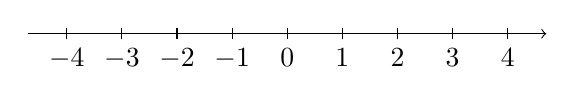
\begin{tikzpicture}[scale=.7]
\draw[->] (-4.7,0) -- (4.7,0);
\foreach \x in {-4,...,4}
\draw (\x,.1) -- (\x,-.1) node[anchor=north] {$\x$};
\end{tikzpicture}
\]
Noen av tallene er \emph{hele tall}, slik som $4$ eller $-17$
eller~$3856$.  Innimellom disse tallene kan vi plassere \emph{brøker},
slik som $1/2$ eller $11/7$ eller $-5/4$.  Tallene som kan skrives som
brøker kalles også for \emph{rasjonale tall}.  (De hele tallene er
forresten også rasjonale, siden de kan skrives som brøker: Tallet
$3856$ er det samme som $3856/1$.)

Og så finnes det
desssuten tall på tallinjen som \emph{ikke} kan skrives som brøker; de
kalles \emph{irrasjonale tall}.  Noen eksempler på slike tall er
$\sqrt{2}$ og~$\pi$.

Totalt kaller vi alle tallene på tallinjen for \emph{reelle tall}.
Det er et litt pussig begrep, som later til å antyde at disse tallene
finnes på ordentlig, i motsetning til andre tall som ikke finnes på
ordentlig.  Men det er nå engang det begrepet som har blitt
innarbeidet, så vi får bare bruke det uten å dvele for mye ved hva det
høres ut som.

Mengden av reelle tall har sitt eget symbol: $\R$.  Vi kan dermed si
at for eksempel tallet $-8/17$ er et \emph{element} i mengden~$\R$, og
det skriver vi slik:
\[
-\frac{8}{17} \in \R
\]

Når vi tegner det todimensjonale planet, så har vi to akser som hver
tilsvarer den reelle tallinjen:
\begin{center}
\begin{tikzpicture}[scale=.7]
\draw[->] (-3.5,0) -- (3.5,0);
\draw[->] (0,-3.5) -- (0,3.5);
\foreach \x in {-3,-2,-1,1,2,3}
\draw (\x,.1) -- (\x,-.1) node[anchor=north] {$\x$};
\foreach \y in {-3,-2,-1,1,2,3}
\draw (.1,\y) -- (-.1,\y) node[anchor=east] {$\y$};
\end{tikzpicture}
\end{center}
Det er vanlig å skrive $\R^2$ for mengden av alle punkter i planet.
Vi tenker på punktene i planet som vektorer, så for oss betyr $\R^2$
mengden av alle todimensjonale kolonnevektorer.  For eksempel er
vektoren $(3,2)$ et element i mengden $\R^2$, og det kan vi skrive
slik:
\[
\vv{3}{2} \in \R^2
\]

Tilsvarende skriver vi $\R^3$ for mengden av alle tredimensjonale
kolonnevektorer, og mer generelt skriver vi $\R^n$ for mengden av alle
$n$-dimensjonale kolonnevektorer.

\smallskip
I hver slik mengde av vektorer finnes det én veldig spesiell vektor,
nemlig \emph{nullvektoren}, som består av bare nuller:
\[
\0 = \vvvv{0}{0}{\vdots}{0}
\]
Her tillater vi oss å være litt slurvete med notasjonen.  Det er
selvfølgelig ikke den samme nullvektoren i $\R^2$, $\R^3$, $\R^4$ og
så videre, men vi kaller alle nullvektorene for~$\0$, så lenge det går
frem av konteksten hvilken av dem det er vi snakker om.
Hvis vi snakker om vektorer i~$\R^2$, så er det dette som er
nullvektoren:
\[
\0 = \vv{0}{0}
\]
Men hvis vi snakker om vektorer i~$\R^3$, så er det:
\[
\0 = \vvv{0}{0}{0}
\]

Det er flere ting som er spesielt med nullvektoren.  Én ting er at
hvis vi tar en hvilken som helst vektor $\v$ i $\R^n$ og ganger den
med tallet~$0$, så blir resultatet alltid nullvektoren:
\[
0 \v = \0.
\]
En annen ting er at nullvektoren er den eneste vektoren som vi ikke
kan tenke på som en pil, for den har ingen retning.

% TODO ordne litt i denne seksjonen, avslutte annerledes?


\kapittelslutt
